\paragraph{Tijdsduur}
Net zoals bij native kijken we enkel naar het CPU en geheugen gebruik tijdens 
het afspelen van audio en video.

\paragraph{CPU \& geheugen}
\begin{figure}[H]
    \centering
    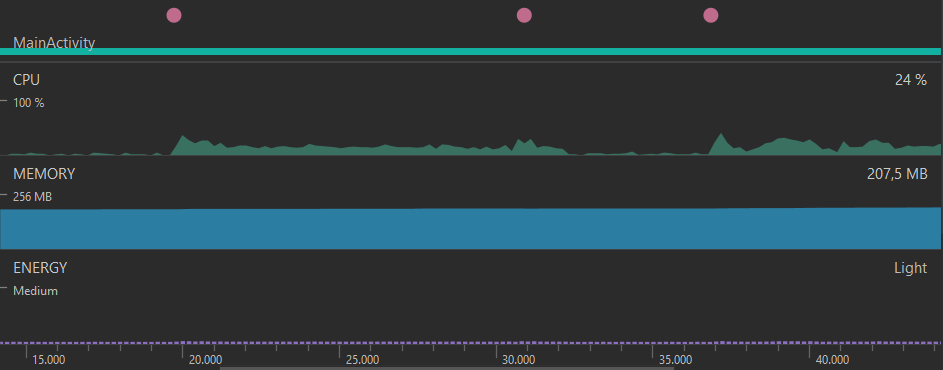
\includegraphics[height=0.3\textheight]{mediaPerformantieCross.png}
    \caption{Overzicht CPU en geheugen gebruik tijdens het afspelen van audie en video bij React native.}
\end{figure}
Op de grafiek kunnen we zien dat bij het eerste klik event voor het starten van de audio het 
CPU gebruik stijgt tot 42\% en daarna afzakt naar een wisselend gebruik van 15 - 25\%. Bij het
tweede klik event voor het pauzeren van de audio stijgt het CPU gebruik tot 35\%. 
Bij het derde klik event voor het starten van de video stijgt het CPU gebruik tot 43\% en 
blijft dan schommelen tussen 10 - 35\%. Tijdens het afspelen van de audio en video blijft 
het geheugen gebruik rond de 207MB hangen. Er is dus geen verschil in
geheugen gebruik bij het afspelen van audio of video en het inactief zijn van de applicatie.
